% ============================================================
% IEEE Wireless Communications Magazine — Special Issue
% "Agentified Embodied AI for Mobile Edge General Intelligence"
% Submission deadline: 1 June 2026
%
% Single-file source: all sections, abstract, biography in this file.
% Bibliography in refs.bib.
% Figures go in figures/ subdirectory.
%
% =========== STYLE NOTES FOR THE TRIM/POLISH PASS =============
% 1. Em-dash overuse: the draft currently uses "---" heavily for
%    parenthetical asides. During the shortening pass, rewrite to
%    avoid em dashes: prefer commas, periods, or sentence splits.
%    Reserve em dashes for genuinely emphatic interruptions (rare).
% 2. Match IEEE magazine sentence style: tight, declarative, active
%    voice. Avoid hedged academic phrasing ("we argue," "it should
%    be noted") and long nested parentheticals. Tutorial register
%    aimed at the wireless reader who is not a deep ML specialist.
% 3. Target after trim: ~4500 words across §I–§VI (magazine guideline).
%    Measured 2026-05-21 with `texcount -inc -sum main.tex`:
%    4527 words in body, 4744 sum (incl. headers + captions, excl.
%    bio and acknowledgements). After SI reframing (intro tutorial
%    paragraph + §V edge-deployment item + privacy expansion), the
%    body grew by ~400 words. Magazine-register tightening pass
%    (Part B of plan) aims to recover that.
% ==============================================================
% ============================================================

\documentclass[journal]{IEEEtran}

\usepackage{cite}
\usepackage{graphicx}
\usepackage{amsmath}
\usepackage{url}
\usepackage{xcolor}
\usepackage{xspace}
\usepackage{tikz}
\usetikzlibrary{positioning, fit, arrows.meta, calc}

% Convenience commands for drafting placeholders
\newcommand{\todo}[1]{\textcolor{red}{\textbf{[TODO: #1]}}}
\newcommand{\tbd}[1]{\textcolor{blue}{[#1]}}

\graphicspath{{figures/}}

\begin{document}

% ============================================================
\title{Deploying LLM Algorithm-Discovery Agents at the Wireless Edge: Hybrid Patterns and Trade-offs}

\author{
Jimmy~J.~Nielsen,~\IEEEmembership{Senior~Member,~IEEE}
\thanks{J.~J.~Nielsen is with the Department of Electronic Systems, Aalborg University, Denmark (e-mail: jjn@es.aau.dk).}
}

\markboth{IEEE Wireless Communications Magazine, Special Issue on Agentified Embodied AI for Mobile Edge General Intelligence, 2026}{Nielsen: Deploying LLM Algorithm-Discovery Agents at the Wireless Edge}

\maketitle

% ============================================================
\begin{abstract}
An emerging direction for AI at the wireless edge embeds algorithm design inside the deployed system rather than confining it to offline R\&D: large language model (LLM) agents propose, implement, and evaluate candidate wireless algorithms as part of normal operation, on hardware that runs alongside the system itself. Reaching this point is currently blocked at the deployment layer. Agent loops capable of competitive algorithm discovery today rely on either frontier closed-weight cloud models or open-weight models that demand shared HPC access, neither of which fits an edge platform's footprint. We describe a hybrid cloud--local deployment that decomposes the agentic loop along its natural traffic asymmetry: a frontier cloud LLM serves the sparse strategic \emph{manager}, while a compact open-weight model on a single workstation serves the dense implementation-intensive \emph{agent}. On the link-adaptation task from a recent algorithm-discovery framework, the hybrid exceeds the fine-tuned outer-loop link adaptation (OLLA) baseline by 1.2\,\% and the published 120\,B-parameter open-weight reference by 1.9\,\% in ten generations, lands within 2.1\,\% of the frontier closed-weight reference, and does so at roughly an order of magnitude lower cloud spend. We further contribute the first per-generation convergence analysis on this task and show that \emph{manager} model quality, not agent model choice, dominates both final score and convergence speed, with direct implications for resource-aware deployment of LLM design agents on edge-class hardware.
\end{abstract}

\begin{IEEEkeywords}
Agentified embodied AI, mobile edge intelligence, large language model agents, wireless algorithm discovery, link adaptation, hybrid cloud--edge inference, resource-aware deployment, vLLM.
\end{IEEEkeywords}

% ============================================================
\section{Introduction}
\label{sec:intro}

\begin{figure*}[!t]
\input{figures/fig1-architecture}
\caption{LLM deployment architectures for agentic algorithm discovery.}
\label{fig:architecture}
\end{figure*}

\IEEEPARstart{A}{gentic} AI is making its first appearances in the wireless workflow. Coding and retrieval agents already draft prototypes and reproduce published results, and a more recent class of \emph{algorithm-design} agents proposes, implements, and evaluates candidate algorithms from a problem description and an evaluator alone, a pattern established for mathematics by FunSearch~\cite{romeraparedes2024funsearch} and extended to broader scientific and algorithmic discovery by AlphaEvolve~\cite{novikov2025alphaevolve} and AI~Scientist~\cite{lu2024aiscientist}. The recent \emph{AI Telco Engineer} framework~\cite{aitaoudia2026aite} carries this paradigm into wireless, generating channel-estimation and link-adaptation algorithms competitive with classical baselines in a few hours of compute. As the broader push toward agentified embodied AI at the wireless edge gathers momentum~\cite{TODO_si_framing}, the same agents that today sit in the research lab are expected to move toward edge platforms tomorrow. Whether they get there is a question of deployment economics: an agent that needs a multi-GPU cluster or hundreds of dollars of cloud spend per task is not a candidate for any edge-scale rollout.

The class of agentic system at issue here pairs two LLM roles in a closed loop. A \emph{manager} reads the problem description and a running summary of prior attempts, then proposes new algorithmic ideas. For each idea, one or more \emph{agents} write code, run an evaluator that scores the candidate against a target metric, and iterate on errors. The manager updates its summary at the end of each generation and proposes the next batch. Across generations the loop searches the implementation space without manual guidance, in the spirit of evolutionary program search but driven by LLM-emitted reasoning~\cite{yao2023react, schick2023toolformer} rather than mutation operators. The field is now beginning to ask explicitly how much of wireless R\&D such loops can automate~\cite{bjornson2026automating, bariah2024llmtelecom, zhou2024llmtelecomsurvey}, and the answer depends on the deployment economics of the underlying AI.

The deployments demonstrated so far sit at two extremes. Frontier closed-weight cloud models such as GPT-5.4 deliver the strongest results~\cite{aitaoudia2026aite} but accumulate substantial cloud-API spending across hundreds of multi-turn agent sessions. Open-weight alternatives such as GPT-OSS 120B require around 240\,GB of GPU memory in BF16, forcing a multi-GPU server or cluster. Either path is incompatible with the resource-aware co-design that the wireless-edge agentic AI programme calls for: too expensive for a sustained per-edge-node footprint, or too memory-hungry for any realistic edge platform.

The manager--agent decomposition that defines this class of frameworks also defines a natural deployment decomposition: the two roles differ by roughly an order of magnitude in call volume, in input context size, and in the kind of capability they require. Strategic synthesis benefits sharply from frontier scale; implementation of well-scoped code does not. The same decomposition generalises to hierarchical embodied-agent settings, where a sparse high-capability planner coordinates many constrained edge-served executors, a structure increasingly central to multi-agent edge intelligence frameworks. We develop these constraints in detail in \S\ref{sec:hybrid}.

Related framings of wireless-LLM systems (e.g., WirelessLLM~\cite{shao2024wirelessllm}) treat the LLM as the algorithm itself rather than as a tool for discovering algorithms. We instead extend the discovery-loop paradigm from~\cite{aitaoudia2026aite} and place it inside the SI's broader programme of agentified embodied AI at the wireless edge, where the question of \emph{where} an agentic loop runs is as binding as how well it performs. Evaluating on the link adaptation task introduced in~\cite{aitaoudia2026aite}, our contributions are:

\begin{itemize}
    \item \textbf{Deployment-pattern comparison (\S\ref{sec:hybrid}--\S\ref{sec:case}).} We characterise three deployment patterns (fully-cloud, fully-local, and a hybrid that exploits the traffic asymmetry between the two roles) across a range of manager and agent model pairings, and quantify the spectral-efficiency vs.\ cloud-cost trade-off of each. The resulting frontier is a quantitative proxy for the deployment-feasibility envelope that the edge-AI literature has so far reasoned about only qualitatively.
    \item \textbf{Per-generation convergence analysis (\S\ref{sec:case}).} The original paper~\cite{aitaoudia2026aite} reports only final scores. We give the first per-generation analysis for this task and find that manager model quality is the dominant factor in both the final score and how many generations are needed to reach a competitive algorithm. For edge-style deployments the implication is direct: investing scarce compute on the planner side pays off more than scaling the executor.
    \item \textbf{Manager--agent compatibility (\S\ref{sec:agentmodel}).} Under a strong manager, two compact open-weight agents with very different code-generation profiles reach indistinguishable scores, but a poorly matched pairing collapses the run. Agent per-generation success rate is a reliability proxy, not a final-score predictor, with implications for any embodied setting that mixes cloud planners and edge executors of different families.
\end{itemize}

Section~\ref{sec:background} reviews the agentic loop. The hybrid architecture and its alternatives appear in \S\ref{sec:hybrid}, the link-adaptation case study in \S\ref{sec:case}, and open challenges for edge deployment in \S\ref{sec:open}.

% ============================================================
\section{Background: LLM Agent Loops for Wireless Algorithm Discovery}
\label{sec:background}

The agentic framework on which our work builds~\cite{aitaoudia2026aite} instantiates a two-tier evolutionary optimisation loop. Each generation, the manager LLM proposes several algorithmic ideas given the problem description and the cumulative results of prior generations, and summarises agent outcomes once the generation completes. An agent LLM, given a single assigned idea and an isolated Docker workspace with code-editing and evaluation tools, implements a Python solution that the framework's evaluator scores against a held-out instance distribution. The agent operates in the interleaved-reasoning-and-acting style of ReAct~\cite{yao2023react} and invokes tools in the manner of Toolformer~\cite{schick2023toolformer}. Several agents run concurrently per generation (multiple agents per idea, so that an unlucky implementation does not waste the idea), capped by a per-agent wall-clock timeout; the best-scoring solution is preserved across generations.

The two roles have very different traffic profiles. The manager issues roughly 11 calls per generation: one idea-generation call with moderate context, plus one short summary call per completing agent. Each agent then makes a multi-turn code-write--evaluate--debug loop of 5--15 calls per session, with input contexts that grow from a few thousand tokens on the first turn to ten to fifteen thousand by the last. In aggregate the agent role accounts for ${\sim}90\,\%$ of LLM calls and an even larger share of input tokens. This sparse-manager / dense-agent asymmetry is what the next section's deployment decomposition exploits.

We focus throughout on the framework's \emph{link adaptation} task. The agent must implement a Modulation and Coding Scheme (MCS) selection controller that, given recent Hybrid Automatic Repeat reQuest (HARQ) feedback and the history of acknowledged MCS indices, maximises long-term spectral efficiency (bps/Hz) over 50 signal-to-noise-ratio (SNR) trajectories of 3000 slots each, generated by ray tracing over a Munich urban scene using Sionna~\cite{sionna}, subject to a long-term block-error-rate constraint of 10\,\%. To bound what the agent must discover from scratch, two helper functions (an SNR-to-per-MCS-BLER mapping and a highest-MCS-satisfying-target-BLER selector) are injected into its workspace at evaluation time. The OLLA~\cite{sampath1997olla}, GPT-5.4, and GPT-OSS 120B reference scores reported in~\cite{aitaoudia2026aite} serve as external baselines, reproduced numerically in \S\ref{sec:case}.

% ============================================================
\section{Hybrid Cloud--Local Architecture}
\label{sec:hybrid}

Fig.~\ref{fig:architecture} contrasts the two architectural patterns at the heart of this design choice. A \emph{single-endpoint} deployment serves both manager and agent calls from the same LLM. This pattern admits two ends of the cost spectrum: a \emph{fully-cloud} configuration is capable but expensive because the dense agent traffic dominates token consumption; a \emph{fully-local} configuration incurs no per-call cost but constrains the manager to whatever model fits on local hardware. The \emph{split-endpoint} pattern we propose places each role on its own endpoint, sized to its traffic profile. The \emph{hybrid} variant we adopt as the headline configuration is the natural sweet spot: a frontier cloud LLM serves the sparse manager role at modest dollar cost, while a compact open-weight model running locally absorbs the dense agent traffic at zero marginal cost per call.

\subsection{Why split the roles?}
\label{sec:asymmetry}

The traffic asymmetry of \S\ref{sec:background} makes a single-endpoint deployment expensive or impractical on workstation hardware. The dominant constraints are \emph{memory} (an open-weight model competitive with frontier cloud APIs needs HPC-class GPU memory, not a workstation), \emph{concurrency} (the framework runs multiple agents in parallel; without an efficient serving stack with continuous batching~\cite{yu2022orca, kwon2023vllm}, wall-clock per generation scales with agent count), and \emph{cloud cost} (a fully-cloud deployment accumulates millions of tokens per ten-generation run, dominated by the dense agent role). Splitting the roles across distinct endpoints, a strong manager on a sparse cheap channel and a competent agent on a dense free channel, decouples the cost of the two and lets each be sized independently.

\subsection{Hardware landscape: edge to workstation}
\label{sec:hwlandscape}

Single-machine unified-memory hardware capable of hosting a compact open-weight agent now spans three tiers, sketching the path along which a workstation-class deployment can shift toward the edge:

\begin{itemize}
    \item \textbf{On-platform edge SoCs.} The NVIDIA Jetson family ranges from the entry-level Jetson Orin Nano (8\,GB LPDDR5 at 102\,GB/s) to the Jetson AGX Orin (up to 64\,GB LPDDR5 at 204\,GB/s); the upcoming NVIDIA IGX Thor brings Grace--Blackwell-class silicon (${\sim}128$\,GB LPDDR5X at 273\,GB/s, comparable to the DGX Spark) into an industrial edge enclosure. These target embedded and ruggedised deployments such as vehicular gateways, UAV controllers, and on-radio-unit installations. At the Nano end, the 26\,B / 30\,B agent models used in this study do not fit in native precision; smaller MoE variants such as Gemma4 E2B / E4B (effective 2--4\,B activations) fit at 4-bit quantisation today.
    \item \textbf{On-premises edge servers.} Compact rack-mount edge servers such as the Lenovo ThinkEdge SE455 V3 (dual NVIDIA L4 GPUs, 2\,$\times$\,24\,GB GDDR6 at ${\sim}300$\,GB/s per GPU) suit RAN-side aggregation points and small regional sites that aggregate traffic from many on-platform nodes.
    \item \textbf{Research workstations.} The NVIDIA DGX Spark (GB10 Grace--Blackwell, 128\,GB LPDDR5X at 273\,GB/s) used in this study, the Apple Mac Studio M3 Ultra (up to 512\,GB at 819\,GB/s), and AMD Ryzen AI Max+ 395 mini-PCs (128\,GB at 256\,GB/s) are the lab-grade analogues. At this tier the choice is shaped as much by software ecosystem (CUDA, MLX, ROCm) as by raw silicon.
\end{itemize}

We use the DGX Spark\footnote{Product pages: \url{https://www.nvidia.com/en-us/products/workstations/dgx-spark/}; \url{https://www.nvidia.com/en-us/autonomous-machines/embedded-systems/jetson-orin/}; \url{https://www.nvidia.com/en-us/edge-computing/products/igx/}; \url{https://www.lenovo.com/us/en/p/servers-storage/servers/edge/thinkedge-se455-v3/}. All accessed 2026-05-17.} because its CUDA stack hosts vLLM directly and the GB10 SoC's native FP8 and FP4 tensor cores open NVFP4 (a 4-bit native floating-point quantisation supported by the GB10 SoC) as a path to fitting larger models on the same memory footprint. The same Grace--Blackwell silicon class is what the IGX Thor edge enclosure will carry, which is what makes the measurements reported here transferable to edge-class hardware. 

\subsection{Concurrent serving of local agents}

The agent endpoint is a vLLM~\cite{kwon2023vllm} server hosting two compact sparse Mixture-of-Experts (MoE) models: Gemma4-26B-A4B-it\footnote{\url{https://ai.google.dev/gemma}. Accessed: 2026-05-17.} and Qwen3-30B-A3B\footnote{\url{https://huggingface.co/Qwen/Qwen3-30B-A3B}. Accessed: 2026-05-17.}. MoE~\cite{fedus2022switch} decouples memory footprint (scales with total parameters) from inference latency (scales with active parameters), which is exactly the trade we want at the workstation scale. Two vLLM features then exploit the agentic loop's structure to extract near-linear throughput scaling with agent count: \emph{prefix caching} (the shared system prompt is prefilled once and reused across all agents that hit the same prefix, amortising roughly 90\,\% of prefill compute on our workload) and \emph{continuous batching}~\cite{yu2022orca} (concurrent agent decode steps are merged at token granularity into the same forward pass, amortising weight-fetch bandwidth across the batch). On the DGX Spark with Gemma4, single-agent throughput is ${\sim}13$\,tok/s and five-concurrent-agent aggregate throughput is ${\sim}64$\,tok/s, near-linear scaling that meets the framework's parallelism needs.

We cap concurrency at five agents because the ${\sim}70$\,GB available after Gemma4's BF16 weights hosts a 32\,K-context KV cache for five sessions with runtime headroom; we keep the same cap for the lighter Qwen3 (${\sim}30$\,GB weights) for direct comparability. Gemma4-26B-A4B-it is served at BF16 throughout the study to remove quantisation as a confound when comparing against the full-precision GPT-5.4 and GPT-OSS 120B baselines of~\cite{aitaoudia2026aite}; Qwen3-30B-A3B-FP8 is served at FP8, the precision in which it ships.

\subsection{Manager endpoint}

The hybrid and fully-cloud configurations route manager calls to a cloud API. The headline configuration uses Anthropic's Claude Opus 4.7\footnote{\url{https://www.anthropic.com/claude}. Accessed: 2026-05-17.} because it sits in the same capability tier as the GPT-5.4 used by~\cite{aitaoudia2026aite}; we also run Sonnet 4.6 as a lower-tier point of comparison and Mistral Large as the mid-tier fully-cloud manager. Each cloud endpoint is exposed via a LiteLLM proxy\footnote{\url{https://github.com/BerriAI/litellm}. Accessed: 2026-05-17.} on a local OpenAI-compatible port, so the framework's existing client can address cloud and local endpoints uniformly. Fully-local configurations replace the cloud manager with a second local model: Gemma4-26B (G4-G4) or, for a larger local-manager point, Nemotron-H 123.6B served via Ollama on a second workstation at Q4\_K\_M quantisation (a 4-bit mixed quantisation scheme from llama.cpp) to fit on a single Spark's memory (Ne-G4).



\begin{table*}[t]
\centering
\caption{Achieved performance on the link adaptation task across the configurations considered, ordered by eval SE. Bold marks configurations that exceed the OLLA baseline. A trailing ``*'' denotes runs with knowledge-state consolidation disabled.}
\label{tab:results}
\footnotesize
\setlength{\tabcolsep}{4pt}
\begin{tabular}{lllcrrrr}
\hline
Configuration & Manager & Agents & Cloud model & Gens & Best gen & Eval SE & vs OLLA \\
\hline
GPT-5.4 ~\cite{aitaoudia2026aite} & GPT-5.4 & GPT-5.4 & Manager+Agents & 10 & --- & 3.5370 & $+3.43\%$ \\
\textbf{Op-G4} & Opus 4.7 & Gemma4-26B & Manager only & 10 & 9 & \textbf{3.4618} & $+1.23\%$ \\
\textbf{Op-G4*} & Opus 4.7 & Gemma4-26B & Manager only & 10 & 8 & \textbf{3.4441} & $+0.72\%$ \\
\textbf{Op-Q3} & Opus 4.7 & Qwen3-30B-A3B & Manager only & 10 & 9 & \textbf{3.4434} & $+0.70\%$ \\
\textbf{ML-CS} & Mistral Large & Codestral & Manager+Agents & 10 & 9 & \textbf{3.4427} & $+0.68\%$ \\
\textbf{ML-ML} & Mistral Large & Mistral Large & Manager+Agents & 10 & 9 & \textbf{3.4296} & $+0.30\%$ \\
OLLA ~\cite{aitaoudia2026aite} & --- & --- & --- & --- & --- & 3.4196 & --- \\
ML-ML* & Mistral Large & Mistral Large & Manager+Agents & 10 & 7 & 3.4069 & $-0.37\%$ \\
So-G4 & Sonnet 4.6 & Gemma4-26B & Manager only & 10 & 8 & 3.4003 & $-0.56\%$ \\
GPT-OSS 120B ~\cite{aitaoudia2026aite} & GPT-OSS 120B & GPT-OSS 120B & Manager+Agents & 10 & --- & 3.3976 & $-0.64\%$ \\
So-G4* & Sonnet 4.6 & Gemma4-26B & Manager only & 10 & 9 & 3.3910 & $-0.84\%$ \\
G4-G4* & Gemma4-26B & Gemma4-26B & None & 20 & 14 & 3.3680 & $-1.51\%$ \\
Ne-G4 & Nemotron-H 123.6B Q4 & Gemma4-26B & None & 16 & 15 & 3.3665 & $-1.55\%$ \\
G4-G4 & Gemma4-26B & Gemma4-26B & None & 20 & 19 & 3.3219 & $-2.86\%$ \\
ML-G4 & Mistral Large & Gemma4-26B & Manager only & 10 & 0 & 3.2365 & $-5.36\%$ \\
Q3-Q3 & Qwen3-30B-A3B & Qwen3-30B-A3B & None & 20 & 9 & 0.8718 & $-74.5\%$ \\
\hline
\end{tabular}
\end{table*}


\subsection{Bounded knowledge state}
\label{sec:consolidation}

The original framework~\cite{aitaoudia2026aite} concatenates per-agent summaries across all completed generations into the manager's input context (up to ${\sim}1000$ tokens per generation), which will exceed the 8--16\,K default of many open-weight serving stacks within a dozen generations; we explicitly raise the Gemma4 vLLM endpoint to 32\,K for this study. To keep manager input bounded for longer runs, we modified the framework to compress accumulated summaries into a structured knowledge state at the end of each generation that retains strong findings (best and moderate approaches, with a ``preserve if metric $\geq 2.0$'' rule), records implementation failures and algorithmic dead-ends to avoid revisiting, and earmarks 2--4 unexplored directions for the next generation. Subsequent generations see the compressed state plus only the latest generation's raw results. The principal motivation is to make long-horizon runs tractable on open-weight managers; we assess the impact on final score in \S\ref{sec:case} by comparing pairs of with/without-consolidation configurations.

% ============================================================
\section{Case Study: Link Adaptation Algorithm Discovery}
\label{sec:case}

We focus on the link adaptation task because it is the cleanest of the framework's three tasks for isolating LLM-only deployment variables: its evaluator runs CPU-only inside the agent container, so it does not contend with the local vLLM endpoint for GPU access, and a fine-tuned OLLA controller~\cite{sampath1997olla} provides a strong external baseline.

We compare fully-local, fully-cloud, and hybrid configurations using state-of-the-art models in each tier, and study the impact of the proposed knowledge-state consolidation by running pairs of with-vs-without configurations.




\subsection{Experimental setup}

We run the framework at the same iteration scale as~\cite{aitaoudia2026aite}: ten (or more) generations of ten agents per generation, with five ideas per generation and two agents per idea. Each agent runs in an isolated Docker container for at most 900 seconds. The evaluator scores each draft on 50 ray-traced channel trajectories of 3000 slots each over a Munich urban scene generated with Sionna~\cite{sionna} under a long-term BLER constraint of 10\,\%. We additionally re-evaluate each generation's running-best workspace on a held-out set of 50 separate trajectories drawn from the same scene; the held-out eval-set SE is what populates Table~\ref{tab:results} and the y-axis of every figure in this section. The fully-local configuration is extended to twenty generations because its convergence remained gradually improving past the ten-generation horizon at which the cloud-managed cases had plateaued; the convergence comparison below is therefore conservative for the fully-local case.

Following~\cite{aitaoudia2026aite} we report single-run results per configuration. A full replication of every cell at the iteration scale used here is prohibitively expensive (each cloud-managed cell consumes hours of wall-clock and dollars of API spend; the fully-local cells consume tens of GPU-hours per seed), so we take two compensating steps. First, as a lower bound on cross-run variance we use the within-run top-10 candidate standard deviation, which ranges from ${\sim}0.002$\,bps/Hz for strong cloud-managed configurations to ${\sim}0.025$\,bps/Hz for weaker ones, and we treat cross-configuration differences below ${\sim}0.02$\,bps/Hz as insignificant. Second, the fully-local G4-G4 row of Table~\ref{tab:results} is reported as the mean across multiple seeds, giving a direct cross-run check on the local-manager ceiling claim that the manager-axis ladder rests on \tbd{insert N and std once G4-G4 reps complete}. The remaining cells stay single-run, with the within-run noise band as the relevant bound on what differences we treat as real.

\textbf{Reproducibility.} The agent endpoint is vLLM \tbd{x.y.z}; the manager proxy is LiteLLM \tbd{x.y.z}; each agent's isolated workspace is a Docker container built from the official AITE base image~\cite{aitaoudia2026aite}. Cloud-API access for the cost figures in \S\ref{sec:case} occurred between 2026-04-XX and 2026-05-17 \tbd{confirm window}. Configuration files, prompts, and run logs are available \tbd{decide between (a) public repo URL or (b) on request from the author before submission}.

\subsection{Final performance: hybrid in the sweet spot}

Table~\ref{tab:results} lists the held-out spectral efficiency for every configuration, ordered by closeness to the frontier closed-weight GPT-5.4 baseline~\cite{aitaoudia2026aite}. The headline result is that the hybrid deployments sit in the sweet spot of the cost-quality frontier: the Opus-managed hybrids (Op-G4, Op-Q3) and the mid-tier fully-cloud configurations (ML-CS, ML-ML) all exceed the fine-tuned OLLA baseline in ten generations, while landing 2--3\,\% below the GPT-5.4 reference. The manager-quality axis admits three empirically distinct tiers: a fully-local ceiling around 3.32--3.37\,bps/Hz across both small (Gemma4-26B) and large (Nemotron-H 123B Q4) local managers; a mid-tier cloud step at 3.40--3.44\,bps/Hz with Mistral Large; and the frontier hybrid result at 3.46--3.48\,bps/Hz with Opus. Scaling the local manager four-fold in active parameters leaves the score essentially unchanged (3.3680 vs.\ 3.3665\,bps/Hz), suggesting the local-manager ceiling is set by reasoning quality rather than raw scale. Fully-local viability depends sharply on the agent model: G4-G4 reaches within 1.5\,\% of OLLA in 20 generations, while the fully-local Qwen3-only Q3-Q3 collapses to a quarter of OLLA. The hybrid recovers the remaining headroom at modest cloud cost regardless of the agent model.

\subsection{Manager quality and convergence}

The published paper~\cite{aitaoudia2026aite} reports only final scores for the link adaptation task. Fig.~\ref{fig:convergence} shows the first per-generation convergence analysis for this task, comparing four configurations that hold the agent constant (Gemma4-26B) and vary only the manager along a tier ladder: fully-local Gemma4-26B (4B active), fully-local Nemotron-H 123B Q4 (12B active), Sonnet~4.6, and Opus~4.7.

\begin{figure}[t]
\centering
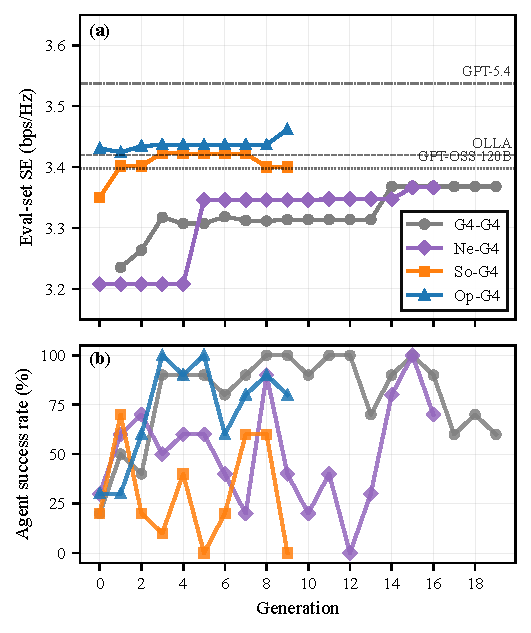
\includegraphics[width=0.95\columnwidth]{fig2-convergence}
\caption{Convergence on the link adaptation task with the agent model held constant (Gemma4-26B-A4B-it) and the manager varying along a tier ladder: fully-local Gemma4-26B, fully-local Nemotron-H 123B Q4, Sonnet 4.6, and Opus 4.7. Top: held-out evaluation-set spectral efficiency of the running-best workspace at each generation. Bottom: agent success rate per generation. Horizontal reference lines mark OLLA, GPT-OSS 120B, and GPT-5.4~\cite{aitaoudia2026aite}.}
\label{fig:convergence}
\end{figure}

The picture has three named axes. The \emph{score ceiling} tracks manager tier: Op-G4 peaks at 3.46\,bps/Hz, So-G4 at 3.40, and both fully-local managers plateau around 3.37, even with twice the generation budget for the local case. The \emph{agent success rate} (lower panel) does likewise: under Opus, 9--10 of 10 agents per generation produce a working solution from generation 3 onward; under Sonnet, success oscillates between 0 and 7 of 10; under the local managers, between 1 and 10, with intermittent collapses to 1 or fewer. Since the agent model is held constant, the differences are attributable to the quality of the manager's ideas, not to agent coding ability. Finally, the \emph{time to a competitive algorithm} also tracks manager tier: Op-G4 is above GPT-OSS 120B at generation 0 and above OLLA from generation 1; So-G4 first touches OLLA at generation 3 but does not sustain it; the fully-local managers never reach OLLA across twenty generations. Each generation consumes a fixed 32--34\,min wall-clock window, so a higher-quality manager extracts a competitive algorithm in fewer hours, not just at a higher ceiling.

\subsection{Agent model choice}
\label{sec:agentmodel}

We evaluate two open-weight MoE agents: Gemma4-26B-A4B (4\,B active, BF16, ${\sim}48$\,GB) and Qwen3-30B-A3B (3\,B active, FP8, ${\sim}30$\,GB).\footnote{Qwen3 is served with its chat template's thinking phase disabled, since the default emits 20\,K+ token chains-of-thought that exhaust the 900-s per-agent timeout before any tool call completes. With thinking off, Qwen3 makes many short tool calls (46--56 per agent at ${\sim}11$\,s each) while Gemma4 makes few long ones (9--15 per agent); per-generation wall-clock is similar.} Two observations across the four manager~$\times$~agent cells in Table~\ref{tab:results} point in the same direction. Under the Opus manager, Op-Q3 and Op-G4 finish within 0.02\,bps/Hz of each other (3.4434 vs.\ 3.4618), inside the within-run noise band. Under the fully-local Gemma4 manager, the Q3-Q3 configuration collapses to 0.87\,bps/Hz, two orders of magnitude below the rest, robust to any plausible inter-run variance. The practical lesson is to prioritise a strong manager before swapping agents: per-generation agent success rate (Qwen3 9--10/10 vs.\ Gemma4 4--7/10) is a reliability proxy, not a final-score predictor.

A counterexample sharpens the lesson. The ML-G4 row (Mistral Large manager paired with Gemma4 agents) reaches only 3.24\,bps/Hz, well below the ML-ML and ML-CS configurations that share the same manager but pair it with Mistral-family agents. The training-set running best is also unusual for this row: it peaks at generation 0 and never improves across the ten-generation budget. We read this as a single-run hint that manager--agent compatibility, not just the strength of either model on its own, can become a binding factor; a controlled replication across managers and agent families is needed before this can be treated as a finding.

\subsection{Effect of consolidation}
\label{sec:consolidation-ablation}

The bounded knowledge state of \S\ref{sec:consolidation} is enabled by default. To isolate its impact on final score we ran three with-versus-without pairs across the three manager tiers (Op-G4, So-G4, ML-ML); the eval-set SE deltas between paired rows in Table~\ref{tab:results} are 0.018, 0.009, and 0.023\,bps/Hz, with consolidation-enabled runs scoring higher in all three cases. All deltas fall within the within-run noise band ($\sim$0.002--0.025\,bps/Hz), so neither a consistent benefit nor a consistent cost can be claimed from a single run per cell. Its principal effect is on \emph{tractability}: Fig.~\ref{fig:consolidation-ablation}(a) compares the manager's input-context size per generation for two Op-G4 runs that differ only in whether consolidation is enabled. Without consolidation the context crosses the 32\,K limit configured on the workstation vLLM by the end of a 10-generation run; with consolidation it stays bounded between 5\,K and 8\,K tokens, which is what makes the longer-horizon runs reported elsewhere in this section feasible. The consequences of exceeding the limit are visible in Fig.~\ref{fig:consolidation-ablation}(b): the oldest workspace cited in the manager's idea proposals for Op-G4* drops abruptly at generation~8, when context truncation begins. Prior to that point the manager consistently references the best workspace found at the start of the run; afterwards it can only cite recent workspaces, having lost the earlier history to silent truncation.

\begin{figure}[t]
\centering
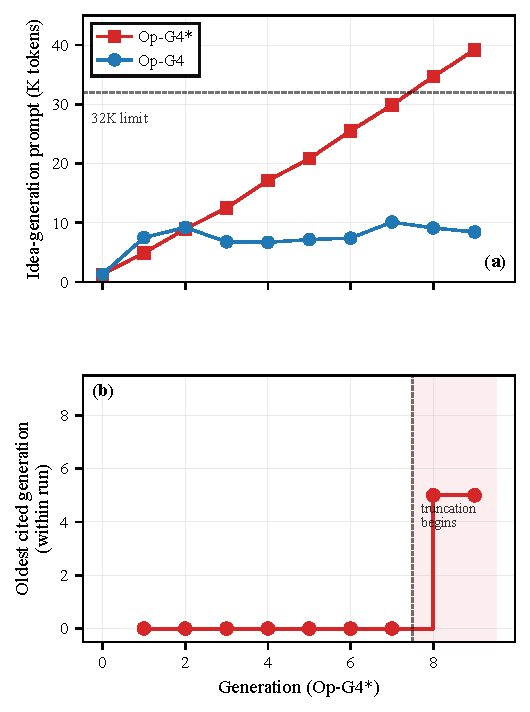
\includegraphics[width=0.95\columnwidth]{fig5-consolidation-ablation}
\caption{(a)~Manager input-context size per generation, Op-G4 with vs.\ without consolidation. The bounded knowledge state holds manager input below ${\sim}8$\,K tokens; the unbounded variant crosses the 32\,K limit at generation~9. (b)~Oldest workspace cited in the manager's idea proposals for Op-G4* (consolidation disabled). The manager references the best early workspace consistently until generation~8, at which point context truncation causes it to lose that history entirely.}
\label{fig:consolidation-ablation}
\end{figure}

\subsection{Cost-quality trade-off}

Fig.~\ref{fig:pareto} plots every measured configuration in Table~\ref{tab:results} on a quality-versus-cost plane, with the per-10-generation approximate cloud cost (USD, log scale) on the horizontal axis and the achieved spectral efficiency on the vertical. Fully-local configurations sit at the left edge at zero marginal cloud cost. Fully-cloud configurations occupy the right side at \$2--\$25 per run. The hybrid deployments fall between the two, at \$0.20--\$1.50 per run, and dominate the cost-quality frontier: Op-G4 at ${\sim}\$1.50$ reaches a higher score than any fully-cloud configuration we measured (ML-ML, ML-CS), and remains within striking distance of the GPT-5.4 reference, which we estimate at one order of magnitude higher cloud cost.

\begin{figure}[t]
\centering
\includegraphics[width=0.95\columnwidth]{fig3-pareto}
\caption{Cost-quality trade-off across configurations from Table~\ref{tab:results}. Hybrid deployments (Opus or Sonnet manager + local Gemma4 agents) dominate the cost-quality frontier across the measured range.}
\label{fig:pareto}
\end{figure}

The measured hybrid manager token usage gives estimated costs of ${\sim}\$0.20$ for So-G4 and ${\sim}\$1.50$ for Op-G4; the measured fully-cloud ML-ML run cost about \$2. Opus 4.7 is roughly $7\times$ more expensive per token than Mistral Large, so a fully-cloud Op-Op run is an estimated \$15--\$25 per 10-generation run.\footnote{Costs are computed from the providers' public per-token pricing on the access date 2026-05-17: Anthropic Claude Opus 4.7 (\tbd{\$/M input}, \tbd{\$/M output}), Anthropic Claude Sonnet 4.6 (\tbd{\$/M input}, \tbd{\$/M output}), Mistral Large (\tbd{\$/M input}, \tbd{\$/M output}). Local Gemma4/Qwen3 agent traffic incurs no per-token cost beyond the workstation's amortised hardware and power.} 

These findings make the hybrid deployment the natural default for workstation-scale agentic algorithm discovery: it reaches within 2\% of the frontier baseline, cuts cloud cost by an order of magnitude, and exceeds OLLA from the first generation.

% ============================================================
\section{Open Challenges and Outlook}
\label{sec:open}

The deployment we have described is a starting point, not an endpoint. Several constraints remain that the community will need to address as agentic algorithm discovery scales beyond proof-of-concept tasks and toward the wireless edge.

\textbf{Deployment at the wireless edge.} The workstation deployment we report is the closest currently-available analogue of an edge platform on which an embodied LLM agent could plausibly run: tens to hundreds of gigabytes of accelerator-addressable memory, single-machine form factor, and a power budget compatible with non-datacentre installations. Moving from workstation toward true edge nodes (vehicular gateways, UAV controllers, on-premises RAN coordinators) tightens every constraint, with stricter thermal and power envelopes, intermittent connectivity for the cloud-served manager, and the need to coordinate many constrained executors against a sparse high-capability planner. Two open questions follow. First, how does agent-side performance degrade as model precision drops from BF16 to native FP4 (the precision that emerging edge SoCs make economical, e.g., NVFP4 on the GB10's tensor cores)? Second, can a single cloud manager schedule and direct multiple geographically distributed edge agents within a single discovery loop, turning today's single-host concurrency into a distributed embodied-agent system? Both are within reach of the pattern reported here, but neither is settled.

\textbf{GPU-in-container barrier.} The link adaptation task evaluates CPU-only, which is what makes it tractable on a workstation that simultaneously serves an LLM on its GPU. The framework's other two tasks (statistics-agnostic and known-covariance channel estimation~\cite{aitaoudia2026aite}) evaluate inside the agent container with Sionna~\cite{sionna}, which requires GPU access from every parallel agent and would contend with the local vLLM endpoint on a single-GPU workstation. Multi-GPU workstations or a separate evaluator host would relieve the contention.

\textbf{Single-task scope.} Our case study focuses on link adaptation. The manager--agent traffic asymmetry that drives the cost finding is structural and should hold across tasks of similar agent-turn complexity. The convergence-speed-by-manager finding is more task-dependent and likely tracks problem complexity.

\textbf{Manager--agent compatibility.} The ML-G4 row in Table~\ref{tab:results} hints that a competent cloud manager and a competent local agent do not automatically combine into a competent hybrid: Mistral Large paired with Gemma4 agents reached only 3.24\,bps/Hz, well below the same manager paired with Mistral-family agents (3.43\,bps/Hz). With a single run per cell, we cannot rule out cross-run noise; but the systematic pattern (training-set running best peaking at generation 0 and never improving) is the kind of failure mode a controlled manager\,$\times$\,agent\,$\times$\,seed sweep would either confirm or dissolve. Until that sweep exists, the safer position is that family-level pairing effects can become a binding factor in distributed embodied-agent settings where planners and executors are typically supplied by different vendors.

\textbf{Long-horizon outlook.} Extending the Op-G4 run from ten to nineteen generations lifted the eval-set SE from 3.4618 to 3.4704\,bps/Hz, closing about 12\,\% of the remaining gap to GPT-5.4. Improvements continue to arrive at the budget boundary, so longer runs likely unlock further gains. The bounded knowledge state of \S\ref{sec:consolidation} makes such extensions tractable on a 32\,K-context manager. Whether the bounded state also \emph{accelerates} convergence is an open question hinted at by late-generation G4-G4 breakthroughs (\S\ref{sec:consolidation-ablation}) but not settled by a single run.

\textbf{Privacy and trust in distributed agentic discovery.} The hybrid architecture already restricts cloud traffic to the manager's distilled outputs and never sends full agent journals, source code, or evaluator outputs to the cloud. This decomposition is a useful starting point for the SI's broader concern with privacy and trustworthiness in distributed embodied-AI collaboration. The link adaptation task is benign, but realistic edge scenarios (operator-specific RAN configurations, customer-segment scheduling policies, infrastructure-vulnerability discovery) carry confidentiality constraints that prevent any task description or evaluator measurement from leaving the operator domain. A fully-local variant remains feasible at the cost of a lower score ceiling (\S\ref{sec:case}); a hybrid variant in which the cloud manager sees only sanitised statistics is an open design problem. Whether such a sanitised channel can support strategic synthesis without leaking task-identifying information is a research question on the path from the lab-grade pattern we report toward zero-trust edge deployments~\cite{TODO_privacy_edge}.

% ============================================================
\section{Conclusion}
\label{sec:conclusion}

LLM-based wireless algorithm discovery does not require a multi-GPU cluster or a substantial cloud bill. We mapped the design space across fully-cloud, fully-local, and hybrid deployments, and found that splitting the agentic loop along its natural traffic asymmetry, with a frontier cloud LLM for the sparse manager role and a compact open-weight model on a single workstation for the dense agent role, exceeds both the OLLA reference and the open-weight cloud baseline for the link adaptation task, lands within 2.1\,\% of the frontier closed-weight cloud result, and does so at an order of magnitude lower cloud cost. The same decomposition surfaces a finding the original paper~\cite{aitaoudia2026aite} did not report: manager model quality, not raw scale and not agent model choice, determines whether the run ever reaches the strong classical reference. Beyond this case study, the planner--executor decomposition is the same one that future embodied-AI deployments at the wireless edge will need to make: scarce strategic capability at one end of an asymmetric channel, dense executor concurrency at the other.

% ============================================================
\section*{Acknowledgements}
The author thanks the team behind the AI Telco Engineer framework~\cite{aitaoudia2026aite} for releasing their code and task definitions, without which the comparisons in this article would not have been possible.
% TODO before submission: add funding sources, infrastructure providers,
% and individual acknowledgements as appropriate. Removed the visible
% \todo macro so the rendered PDF is clean during revision rounds.

% ============================================================
\bibliographystyle{IEEEtran}
\bibliography{refs}

% ============================================================
% TODO before submission of an accepted manuscript: add author photo with \IEEEbiography[{\includegraphics{...}}]{...}.
% For now using \IEEEbiographynophoto so the proof PDF does not render
% the "PLACE PHOTO HERE" placeholder box. Fill the SM elevation year in
% place of the literal "XX" below if known.
% \begin{IEEEbiographynophoto}{Jimmy J.~Nielsen}
% (S'09--M'13--SM'XX) is an Associate Professor with the Department of Electronic Systems, Aalborg University, Denmark. His research interests include reliable wireless communications, low-power IoT, and the application of machine learning and large language models to wireless system design.
% \end{IEEEbiographynophoto}

\end{document}
